\documentclass[prb,preprint]{revtex4-1} 
% The line above defines the type of LaTeX document.
% Note that AJP uses the same style as Phys. Rev. B (prb).

\usepackage{amsmath}  % needed for \tfrac, \bmatrix, etc.
\usepackage{amsfonts} % needed for bold Greek, Fraktur, and blackboard bold
\usepackage{graphicx} % needed for figures
\usepackage{color}
\usepackage{ulem}
\usepackage{multirow}
\begin{document}

% Be sure to use the \title, \author, \affiliation, and \abstract macros
% to format your title page.  Don't use lower-level macros to  manually
% adjust the fonts and centering.

\title{Single-Photon Interference}


\author{Liza Mulder}
\email{emulder@smith.edu}
\affiliation{Department of Physics, Smith College, Northampton, MA 01063}


\author{Isabel Lipartio}
\email{iliparti@smith.edu}
\affiliation{Department of Physics, Smith College, Northampton, MA 01063}


\date{\today}



\begin{abstract}

It has been understood since the 19th century that light displays both wavelike and particle-like properties.  Light beams of differing phase interfere with each other and create observable light and dark fringes, as seen in Young's Double Slit experiment.  At the same time, light can be seen as a particle:  quanta of light, or photons, excite electrons to higher states of energy as seen in the photoelectric effect.  It is unlawful to attempt to classify light as a single entity.  We demonstrate the dual nature of light in the Single Photon Interference Experiment- a variation of Young's Double Slit Experiment.  We use a beam of light and a double slit apparatus, however, in this case, we have confirmation that, within a certain probability, there is only a single photon in flight through the double slit device at any time.  Considering light to be a particle, we would expect to see two single bright fringes projected onto a screen.  However, we do actually see an interference pattern as seen in the Double Slit experiment.  The photons 'interfered with themselves'- the light was both a wave and a particle at once!  In this paper, we discuss the revolutionary implications of this result as well as how we might model these interference patterns.  We fit the Fresnel and Fraunhofer models of interference to our data and discuss the advantages and disadvantages of each.

\end{abstract}

\maketitle % title page is now complete


\section{Introduction} % Section titles are automatically converted to all-caps.
% Section numbering is automatic.

The revolutionary discovery of the dual wave-particle nature of light has been of significance beginning in the 19th century and continuing to today.  Isaac Newton himself believed defining light as a particle-like quantity (calling them corpuscles) would explain light refraction and reflection \cite{newton}.  This idea was, however, superseded in the 19th century by the wave theory of light, due to the significant advances in electromagnetism.  The interference experiments by Young in the early 19th century opposed the ideas of Newton and demonstrated the wavelike nature of light.  Young sent light beams through a single slit and observed diffraction of light waves passing through the slit.  Young sent light beams through two slits and observed resultant interference patterns.  In the latter part of the 19th century, discoveries by Maxwell, Faraday, and Hertz lead to the unification of the theories of electricity and magnetism.  There is a single electromagnetic entity- an electromagnetic wave propagating through the electromagnetic field.  Light was realized to be an electromagnetic wave- a disturbance in an electromagnetic field.  The contemporary theories of light bore little resemblance to the corpuscular theory of Newton.  \cite{david}

However, support for the particle nature of light made a comeback in the early 20th century.  Perhaps the most famous example of this is Einstein's Nobel Prize winning explanation of the photoelectric effect, whose effects absolutely contradicted all predictions from the wave theory of light.  Einstein demonstrated that quanta of light, now called photons, strike the surface of a metal plate and excite electrons to freedom (Cite our modern physics book).  The advent of quantum mechanics- a field based largely off the quantized nature of electromagnetic energy, further explored the particle-like properties of light.  A further example of this is Compton Scattering- a effect where a photon elastically collides with an electron and experiences a shift in wavelength.  

We know now that we can treat light as a particle- photons scatter and collide with matter.  We can also treat it as a wave- light beams constructively and deconstructively interfere with each other.  But, particularly as relatively new physics students, can we call this an acceptable definition of light?  Can we say that we understand light?  The best way to test our understanding and perhaps obfuscate things a little bit is to undertake the Single Photon Interference Experiment.  We will take the same general set up as for the Young Double Slit Experiment:  beam of light, double slit, and means of viewing the output (see Methods section for a detailed description).  However, this time, we will reduce the intensity of light that we can be sure, to within a certain probability, that there is only a single photon in flight through the double slit apparatus at a certain time. \cite{teachspin}

Even recalling the dual nature of light, we still want to insist that there should only be two bright streaks, parallel to the two slits.  We think, incorrectly, that each single photon must 'choose' a slit to pass through, and that is that!  There are no other photons going though the slits and we think that there should be no interference.  

The result of the single photon experiment is, to perhaps our surprise, an interference pattern, just like the one from Young's Experiment!  It seems like the photon 'went through two slits at once', or that it 'interfered with itself'.  The only lawful explanation we can provide at the moment is 'light is more complicated than we thought'.  

In this paper, we perform the Single Photon Experiment and examine the output double slit interference pattern produced by single photon interference.  We fit our output to two different models:  the Fraunhofer model and the Fresnel model, which draw upon different approaches to model the behavior of light.  The Fraunhofer model makes use of the picture of light as a plane wave reaching the two slits and propagating through it as a wave.  The Fresnel model considers the phase variation of an electromagnetic field with position in that field.  The Fresnel model is a sum over multiple paths from one location to another (here, from the source to the detector).  We discuss these models and our found fits in our analysis section.


\section{Methods}

We used the Teach-Spin "2-Slit Interference One Photon at a Time" Apparatus for this experiment.  The apparatus comes with a long black box containing an adjustable light source (with green filter to restrict wavelength and intensity), a 670nm laser source for alignment, four magnetic slit-holders along the length of the box for adding slits in the path of the light, and two detector options at the end: a photodiode (for laser light) and a photomultiplier tube (for lightbulb illumination).  We placed a single columnating slit in the first holder to focus the light from the lightbulb. This created vertical a single-slit diffraction pattern, which we centered on the next set of slits.  In the second slit holder, in the middle of the box, we placed the double-slit, and immediately following that we placed the slit blocker (a wide single-slit) so we could choose to allow light through one slit, both slits, or neither.  At the far end of the box we placed a single slit for the detector slit - by moving this slit holder lengthwise across the channel we could "scan" the interference pattern and measure photon counts at regular intervals.  

Behind the detector slit was a photomultiplier tube (PMT).  The PMT generated an electrical current in response to the arrival of a photon, and adjusting the PMT settings changed the sensitivity - a low setting missed lower-energy photons, but a higher setting generated more noise.  We optimized this setting at 600V.  The short "pulse" from the PMT was translated into a voltage spike, which we sent to the pulse counter interval timer (PCIT).  The PCIT had a "discriminator" which screened out all pulses below a threshold voltage (in order to remove low energy noise, at the expense of some lower-energy photons) - we optimized this setting at 1.5V. The PCIT kept count of how many voltage "pulses" above its threshold voltage it received from the PMT within a 10s, 1s, or 0.1s time interval. More photon detections within the time interval indicated a high light intensity at that position of the detector slit, and photon detection levels near the background indicated a dark fringe in the pattern. By optimizing the apparatus alignment and the PMT and PCIT settings, we obtained a signal to noise ratio of roughly 2000 at the brightest point in the pattern.  

To collect data, we moved the detector slit in increments of 0.1mm across the width of the interference pattern, measuring the photons counted for a 1s interval at each position.  The apparatus came with a micrometer which moved the detection slit holder 0.5mm every turn, and allowed us to read the slit's current position from the barrel.  In this way we could measure the photon counts at different positions.  We repeated this process with the slit blocker in different positions: once blocking the near slit and scanning the single-slit diffraction pattern generated by the far slit, once blocking the far slit and scanning the pattern produced by the near slit, once with both slits unblocked, and once with both slits blocked to get a read of the background.  We did three runs for each position of the slit blocker, to get a measure of the scatter in the results.  Due to the random nature of the phenomena, and the method of data collection, we could not obtain an uncertainty for individual measurements - we instead calculated error from the data for the three runs with the same settings.  We analyzed this data and compared it to two theoretical models with Mathematica.  

\begin{figure}[h!]
\centering
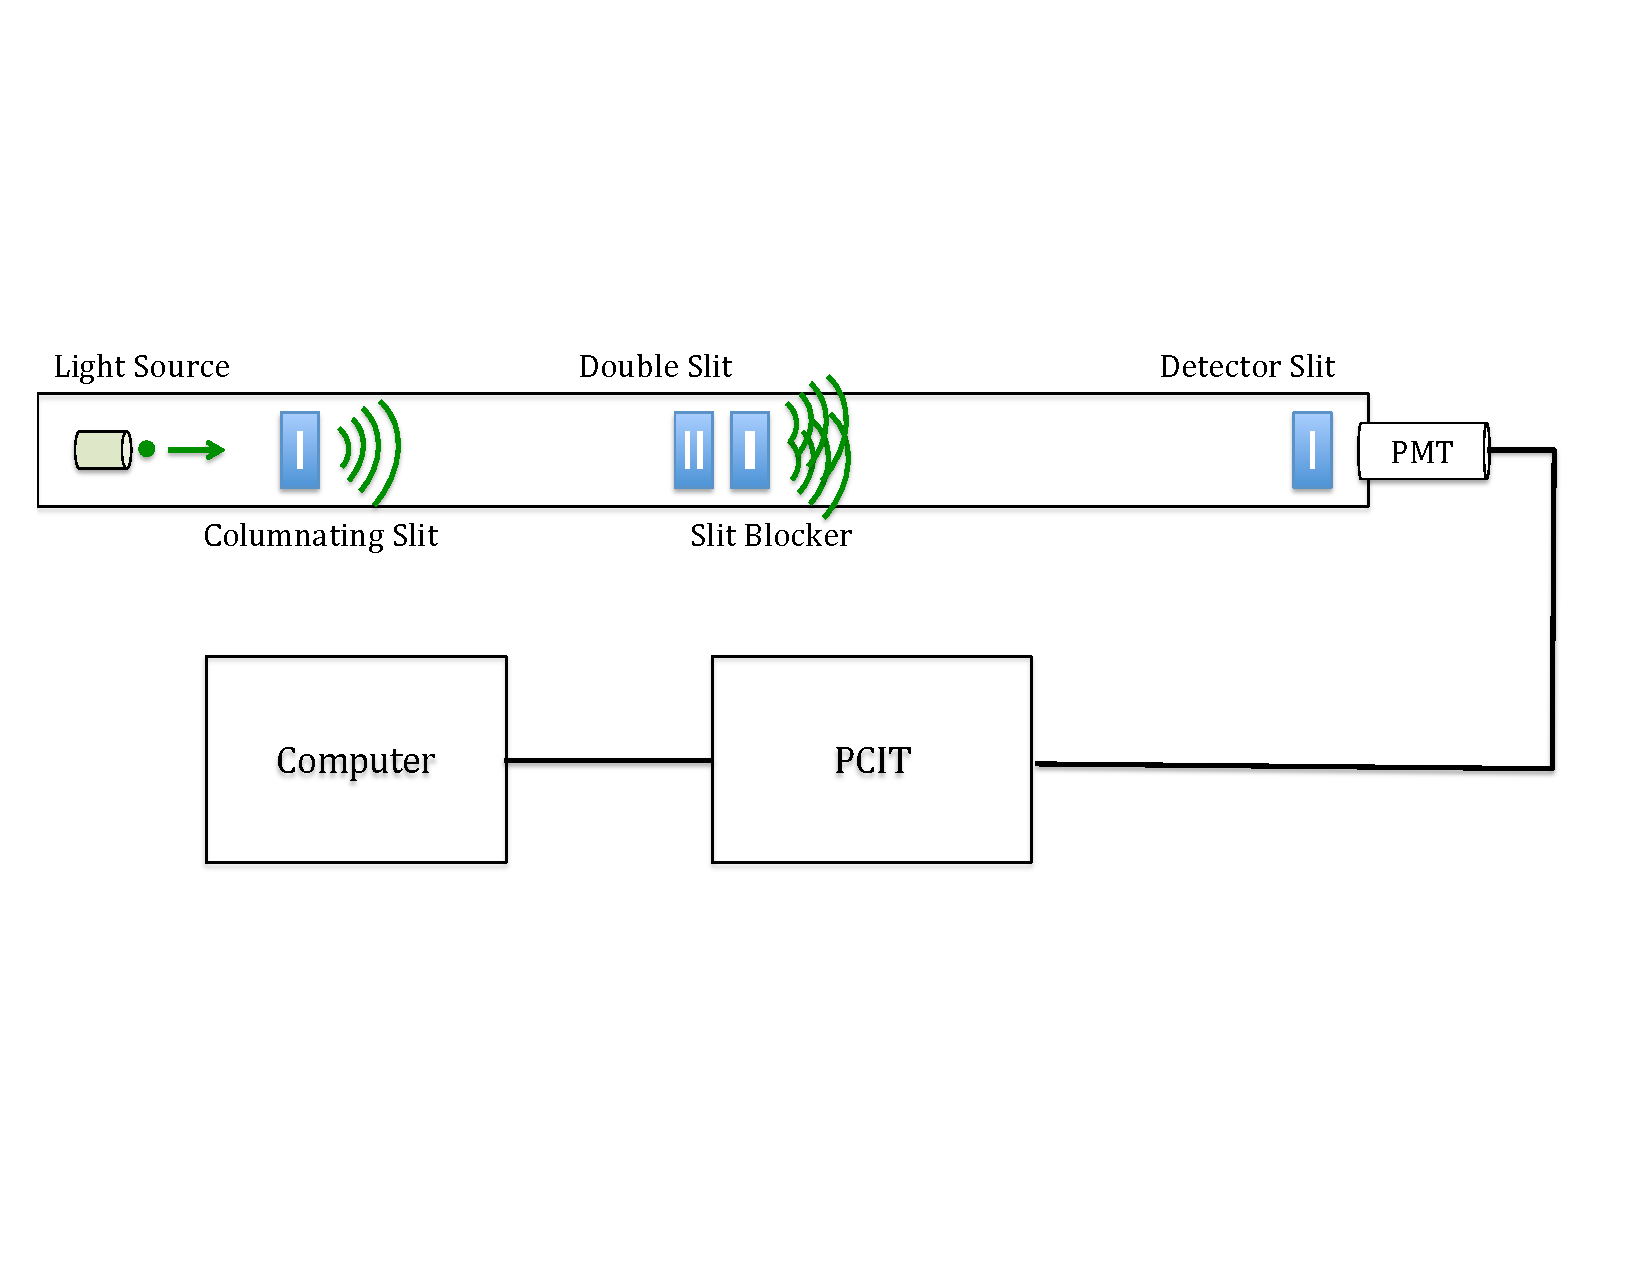
\includegraphics[width=6in]{set-up.pdf}
\caption{Teach-Spin apparatus to measure quantum interference: a 1m-long black box containing an adjustable light source (about 550nm), columnating single slit, double slit, slit blocker, detector slit, and photomultiplier tube (PMT) detector. We sent the PMT output to a pulse-counter interval timer (PCIT), and from there to the computer.}
\label{set-up}
\end{figure}

\section{Results}

The main result of our experiment was that we did indeed see single slit and double slit interference patterns, as we expected.  We then we fit two models to the data, to quantitatively verify our observation and agreement with theory.  Figures ~\ref{double_slit_plot} and ~\ref{single_slits_plot} show the detected light intensity (measured by the number of photon counts per second) at sequential micrometer settings (which give the position of the detector slit). The red data points are our raw data, showing the scatter across three runs, as well as the general trend. The larger, blue data points are the average values with error bars (the mean and standard deviation of the values from the three runs) for each value of position.  Our data has the form of single and double slit diffraction patterns, qualitatively.  In the analysis section we compare our data to two theoretical models. 

\begin{figure}[h!]
\centering
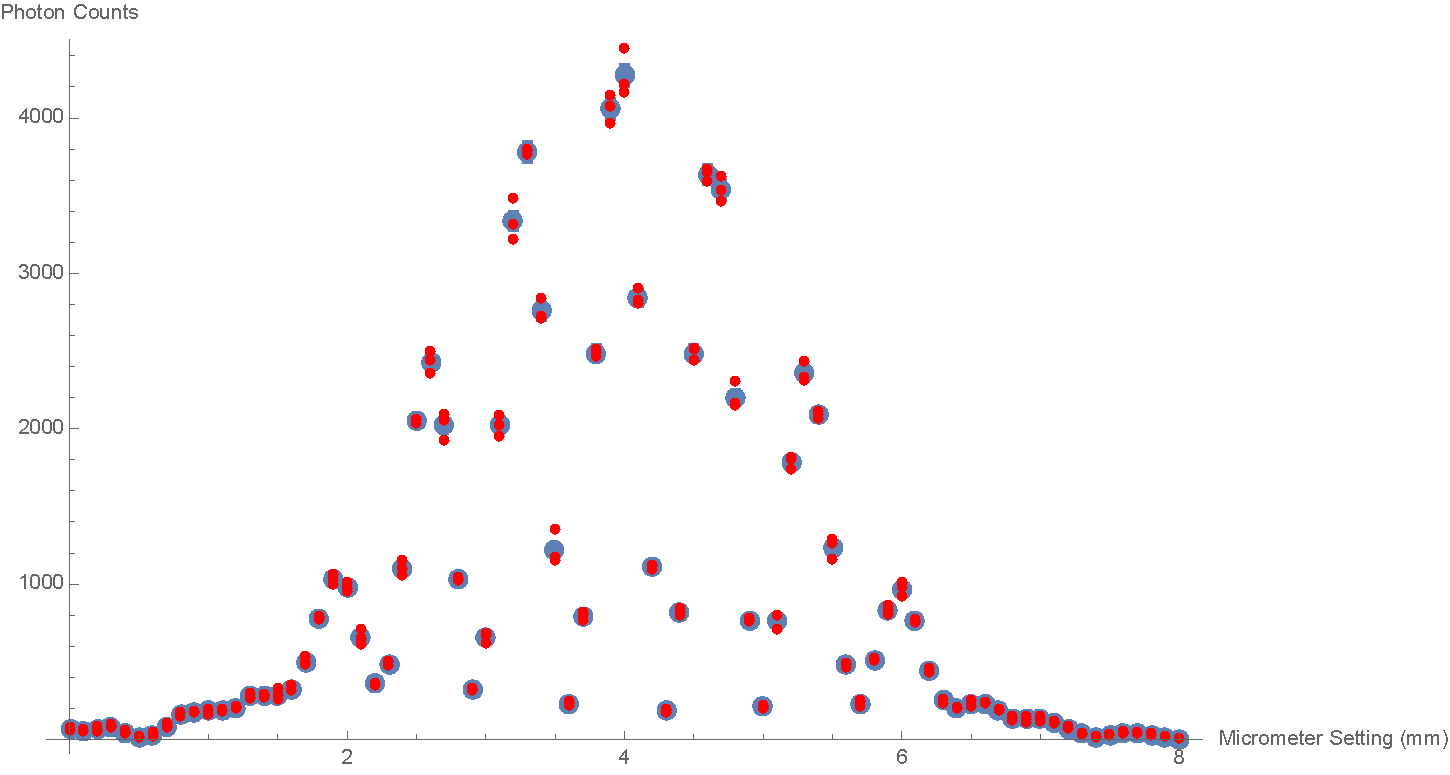
\includegraphics[width=6in]{double_slit_plot.pdf}
\caption{Our data for the double slit pattern.  Raw data is the small red points, averages with standard error are the larger blue points with error bars. }
\label{double_slit_plot}
\end{figure}

\begin{figure}[h!]
\centering
\begin{minipage}[b]{0.45\linewidth}
	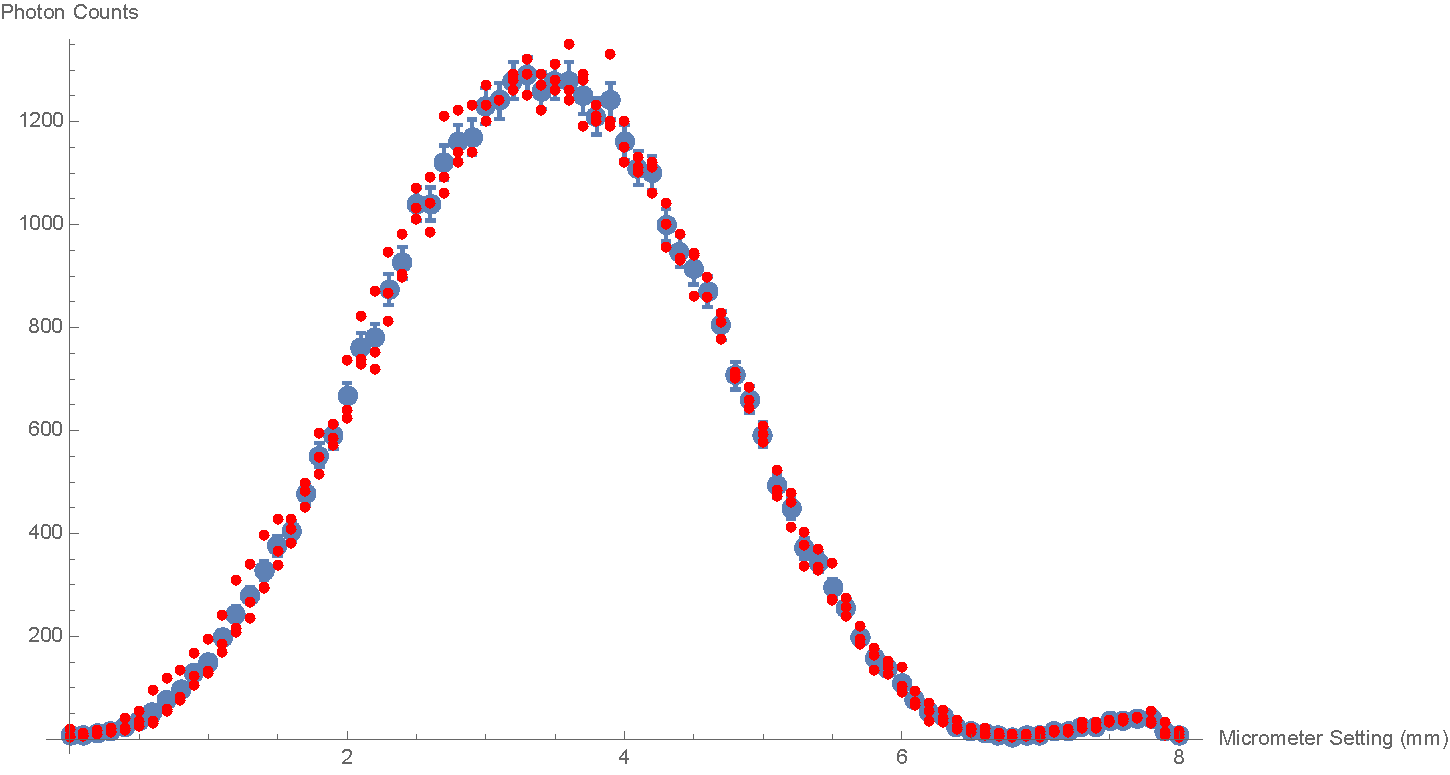
\includegraphics[width=3in]{far_slit_plot.pdf}
\end{minipage}
\quad
\begin{minipage}[b]{0.45\linewidth}
	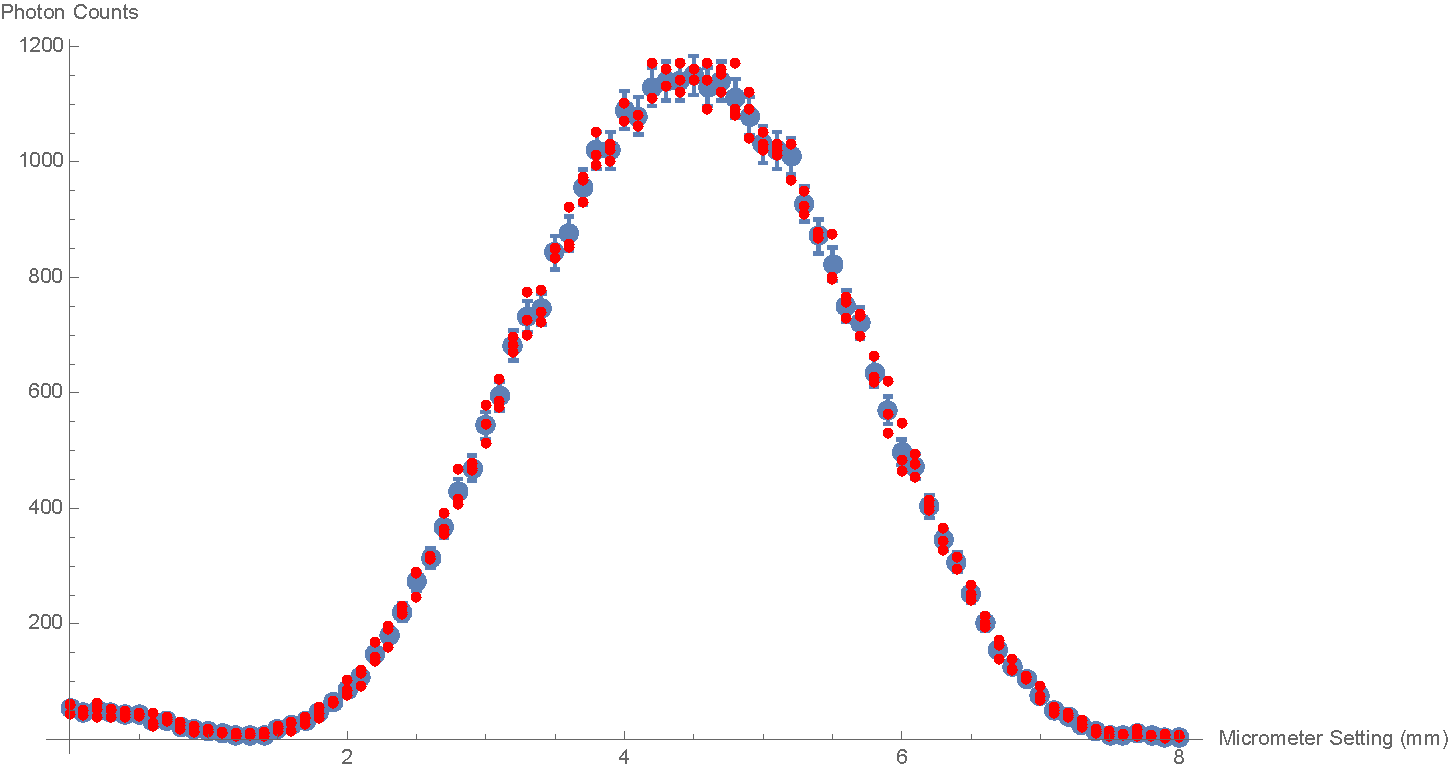
\includegraphics[width=3in]{near_slit_plot.pdf}
\end{minipage}
\caption{Our data for the single slit patterns. Raw data is the small red points, averages with standard error are the larger blue points with error bars. }
\label{single_slits_plot}
\end{figure}

\section{Analysis}

Below, we discuss the two models and our fits, as well as the goodness of these fits and their implications for this experiment and the theory of light.

We calculated fits for both the Fraunhofer Model and the Fresnel Model.  The two are applied in different regimes, determined by the Fresnel number: $F = \frac{a^2}{\lambda L}$.  When $F << 1$ the small slit is far from the detector screen, and the Fraunhofer model applies.  Nearer to the slit, where $F \approx 1$, the Fresnel model is more accurate. ~\cite{wolfram} The Fresnel number for our experiment is roughly $\frac{(0.1mm)^2}{555nm*500mm} \approx 36$.  Therefore the Fresnel model should be more appropriate, though neither is quite right - we would have to use a longer box, a longer wavelength light source, or thinner slits, to make the Fresnel number closer to $1$. 

\subsection{The Fraunhofer Model}

The Fraunhofer Model treats light as a wave and models it's arrival at a plane very far away. This is called "far field." It uses the assumption that the distance between the plane of the slit and the detector plane is much greater than the features of the slits or of the diffraction pattern.  This assumption allows the integral of complex exponentials which exactly describes the situation (shown later in the Fresnel model) to be approximated by the following sinusoidal equations, which are simpler. ~\cite{wolfram}

For the double slit case, the equation simplifies to:
\begin{equation}
I_{double}= I_{0}(\frac{\sin(\frac{\pi a}{\lambda}\sin(\frac{x-x_{0}}{D_{2}}))}{\frac{\pi a}{\lambda}\sin(\frac{x-x_{0}}{D_{2}})})^{2} \times \cos(\frac{\pi d}{\lambda}\sin(\frac{x-x_{0}}{D_{2}}))^{2}
\end{equation}

For the single slit cases, the equations are: 

\begin{equation}
I_{far}= \frac{I_{0}}{4}(\frac{\sin(\frac{\pi a}{\lambda}\sin(\frac{x-x_{1}}{D_{2}}))}{\frac{\pi a}{\lambda}\sin(\frac{x-x_{1}}{D_{2}})})^{2} 
\end{equation}

\begin{equation}
I_{near}= \frac{I_{0}}{4}(\frac{\sin(\frac{\pi a}{\lambda}\sin(\frac{x-x_{2}}{D_{2}}))}{\frac{\pi a}{\lambda}\sin(\frac{x-x_{2}}{D_{2}})})^{2} 
\end{equation}

Where $I_0$ is the amplitude of the central maximum, $a$ is the width of the slits, $x_0$ is the location of the central maximum in the double-slit pattern, $x_1$ is the location of the central max in the far single-slit pattern, $x_2$ is the location of the central max in the near single-slit pattern, $D_2$ is the distance between the slit and the detector, $\lambda$ is the wavelength of the light, $x$ is the position of the detector slit, and $c$ is a vertical offset. 

We fit our data to the Fraunhofer model by plotting our entire data set against the model, using the manufacturer's values for the slit widths, slit separation, and light wavelength, and our observed maximum intensity and central maximum locations.  We then modified these values to try and get a better fit of the function to the data.  As the manufacturer did not give error for most of their parameters, we had to guess at the limits within which we could vary the parameter values.  However, we obtained a good fit for the double slit pattern (with the exception of the very edges), and decent fits for the single slit patterns.  Our single slit data was slightly off because we had not centered the columnated light exactly on the two slits, so one slit had approximately $10\%$ more illumination than the other.  As the fit assumed equal illumination from both slits, the amplitudes did not match.  

\begin{figure}[h!]
\centering
\begin{minipage}[b]{0.45\linewidth}
	\includegraphics[width=3in]{far_slit_Fraunhofer_plot.pdf}
\end{minipage}
\quad
\begin{minipage}[b]{0.45\linewidth}
	\includegraphics[width=3in]{near_slit_Fraunhofer_plot.pdf}
\end{minipage}
\caption{Our data for the single slit patterns with the Fraunhofer formula on top. The parameters we used are in Table ~\ref{parameters}. Raw data is the small red points, averages with standard error are the larger blue points with error bars. }
\label{single_slits_Fraunhofer_plot}
\end{figure}

\begin{figure}[h!]
\centering
\includegraphics[width=6in]{double_slit_Fraunhofer_plot.pdf}
\caption{Our data for the double slit pattern.  Raw data is the small red points, averages with standard error are the larger blue points with error bars. }
\label{double_slit_Fraunhofer_plot}
\end{figure}

\begin{table}[h!]
\centering
\caption{Parameter values for our fits. We started with the values given in the apparatus manual ($a, d, \lambda$), measured ($D_1, D_2$), or estimated from the plots ($I_0, x_0, x_1, x_2, c$).  We then optimized (within the uncertainty for each parameter) to get the Fraunhofer fits as close to the data as possible. }
\begin{ruledtabular}
\begin{tabular}{lc}
Parameter & Fit value       \\
Counts/sec at central max $I_0$     & 4400 counts/sec \\
Slit width $a$       & 0.085 mm        \\
Slit separation $d$       & 0.406 mm        \\
Light wavelength $\lambda$ & 555 nm          \\
Location of central max (double slit) $x_0$     & 3.95 mm         \\
Location of central max (far slit) $x_1$     & 3.45 mm \\
Location of central max (near slit) $x_2$ & 4.45 mm \\
Offset $c$       & 3.6 counts/sec. \\
Distance from columnating slit to diffracting slits $D_1$     & 338 mm          \\
Distance from diffracting slits to detector slit $D_2$     & 500 mm         
\end{tabular}
\end{ruledtabular}
\label{parameters}
\end{table}

\subsection{The Fresnel Model}

The Fresnel model does not use the approximation from the Fraunhofer model, since the detector plane is assumed to be in the "near field," closer to the slits. Therefore the equation is left in it's complex exponential form, and the distances between the slits and between slit and detector become very important.  ~\cite{wolfram} This equation is very difficult to solve, but a computing program such as Mathematica can run the calculation.  

The single slit cases:

\begin{equation}
I_{near}=I_{0}*42.044*|e^{\frac{2 \pi i D_{1}}{\lambda}}*e^{\frac{2 \pi i D_{2}}{\lambda}}*\int_{x_{0}-\frac{d}{2}}^{x_{0}+\frac{d}{2}+a} \! e^{\frac{2 \pi i (x_{0}-y)^{2}}{D_{1} \lambda}}*e^{\frac{2 \pi i (y-z)^{2}}{D_{2} \lambda}} \, \mathrm{d}y |^{2}
\end{equation}

\begin{equation}
I_{far}=I_{0}*42.044*|e^{\frac{2 \pi i D_{1}}{\lambda}}*e^{\frac{2 \pi i D_{2}}{\lambda}}*\int_{x_{0}+\frac{d}{2}}-a^{x_{0}-\frac{d}{2}} \! e^{\frac{2 \pi i (x_{0}-y)^{2}}{D_{1} \lambda}}*e^{\frac{2 \pi i (y-z)^{2}}{D_{2} \lambda}} \, \mathrm{d}y |^{2}
\end{equation}

The double slit case is simply the sum of the waveforms generated by each slit: 
\begin{equation}
I_{double}=I_{near}+I_{far}
\end{equation}

The parameters have the same meanings as in the Fraunhofer model, with the addition of $D_1$, the distance from the columnating slit to the diffracting slit, and with the exception of $x$, $y$, and $z$: $x$ is the location of the columnating slit, $y$ is the location of the diffracting slit, and $z$ is the location of the detector slit.  Figure ~\ref{Fresnel_diagram} shows the parameters and their use in the Fresnel model.  

\begin{figure}[h!]
\centering
\includegraphics[width=4in]{Fresnel_diagram.png}
\caption{The set-up and variables used in the Fresnel Approximation. Note that the variable "Z" in the Fresnel formula is what we've been calling "X" in our other calculations - the position of the detector slit.}
\label{Fresnel_diagram}
\end{figure}

\begin{figure}[h!]
\centering
\includegraphics[width=6in]{double_slit_Fresnel_plot.pdf}
\caption{Our data for the double slit pattern.  Raw data is the small red points, averages with standard error are the larger blue points with error bars. }
\label{double_slit_Fresnel_plot}
\end{figure}

\begin{figure}[h!]
\centering
\begin{minipage}[b]{0.45\linewidth}
	\includegraphics[width=3in]{far_slit_Fresnel_plot.pdf}
\end{minipage}
\quad
\begin{minipage}[b]{0.45\linewidth}
	\includegraphics[width=3in]{near_slit_Fresnel_plot.pdf}
\end{minipage}
\caption{Our data for the single slit patterns with the Fraunhofer formula on top. The parameters we used are in Table ~\ref{parameters}. Raw data is the small red points, averages with standard error are the larger blue points with error bars. }
\label{single_slits_Fresnel_plot}
\end{figure}

After fitting our data, we computed the chi-square value for each fit (see Table ~\ref{chi-square}).  All the values were very large.  By examining the distance of individual points from the fit, however, we realized that the majority actually had small deviations from the line, with a few outliers which weighted the fit.  Even so, from the graphs it is clear that no single set of parameter values allows all the fits to match the data.  We optimized our parameters for the Fraunhofer double-slit fit - as these parameter values were within the uncertainty of what we knew they should be, we kept these parameters.  However, the other fits each had some sort of systematic offset from the line.  

\begin{table}[h!]
\centering
\caption{Reduced chi-square values for our fits. }
\begin{ruledtabular}
\begin{tabular}{cccc}
                            &             & 0mm \textless x\textless 80mm & 20mm \textless x \textless 60mm \\
\multirow{3}{*}{Fraunhofer} & Double Slit &57.67                      & 9.76                         \\
                            & Far Slit    & 3.31                       & 1.16                        \\
                            & Near Slit   & 0.326                       &        0.091           \\
\multirow{3}{*}{Fresnel}    & Double Slit &          155.41               & 86.70                         \\
                            & Far Slit    & 4.80                       & 0.311                         \\
                            & Near Slit   & 4.23                       &1.01                       
\end{tabular}
\end{ruledtabular}
\label{chi-square}
\end{table}


\section{Discussion}

Our biggest question with this experiment was why, while we obtained clear data of the interference patterns, these results deviated from the theoretical model.  In particular the Fresnel model could not be made to fit our data, even with the best estimations of our parameters, and considering we were in the regime of the Fresnel model (detector not very far away), we found this strange. In addition, we observed that the Fresnel model did very well at the very edges of our pattern, while the Fraunhofer model did better in the middle.  We do not know why this was.  

In order to gauge better the fits of the models to the experimental data, we would want to repeat this experiment using smaller incremental turns of the micrometer.  There are large gaps in our plotted fits that could be closed with tighter measurements.  We possibly would want to turn the micrometer by .05 mm instead of .1 mm increments.  

\section{Conclusion}

 
\begin{thebibliography}{3}
 \bibitem{newton}Use of Hamilton's Canonical Equations to Rectify Newton's Corpuscular Theory of Light:  A Missed Opportunity.  Buenker et al, 2004.  Sov. J. Chem. Phys. 22 (2003) 124
 \bibitem{david}Introduction to Electrodynamics, 4th Edition.  David J. Griffiths, 2012.  Addison Wesley.
\bibitem{wolfram}Weisstein, Eric W. Wolfram Science World, "Fraunhofer Diffraction," "Fresnel Diffraction," "Fresnel Number." 2007. 
\bibitem{teachspin} TeachSpin Instruction Manuals.  Two-Slit Interference, One Photon at a Time (TWS1-B).  TWS1B-PCIT1 Instruction Manual. Rev. 1.0 6/2013

\end{thebibliography}
\end{document}
